\documentclass[10pt]{article}
\usepackage[polish]{babel}
\usepackage[utf8]{inputenc}
\usepackage[T1]{fontenc}
\usepackage{amsmath}
\usepackage{amsfonts}
\usepackage{amssymb}
\usepackage[version=4]{mhchem}
\usepackage{stmaryrd}
\usepackage{graphicx}
\usepackage[export]{adjustbox}
\graphicspath{ {./images/} }

\title{V Konkurs matematyczny St@ś }

\author{}
\date{}


\begin{document}
\maketitle
XIV LO im. Stanisława Staszica\\
30 maja 2005 roku

\section*{klasa VI}
Na rozwiazanie poniższych zadań masz 90 minut. Kolejność rozwiazywania tych zadań jest dowolna. Wszystkie zadania sa jednakowo punktowane. Maksymalna liczbę punktów mȯ̇e uzyskać jedynie petne rozwiazanie, z uzasadnieniem i odpowiedzia.\\
Używanie korektora i korzystanie z kalkulatora jest niedozwolone.\\
Zad. 1 Dana jest liczba \(3^{5}+3^{6}+3^{7}+\ldots+3^{2005}\). Oblicz resztę z dzielenia tej liczby przez 2 .\\
Zad. 2 Dane są dwa okręgi styczne zewnętrznie, każdy z nich o promieniu 3 cm . Punkty \(S\) i \(O\) to środki okręgów. Prosta równoległa do prostej \(S O\) przecina okręgi w punktach \(A, B, C, D\), jak na rysunku. Długość odcinka \(B C\) jest równa 2 cm . Oblicz długość odcinka \(A D\).\\
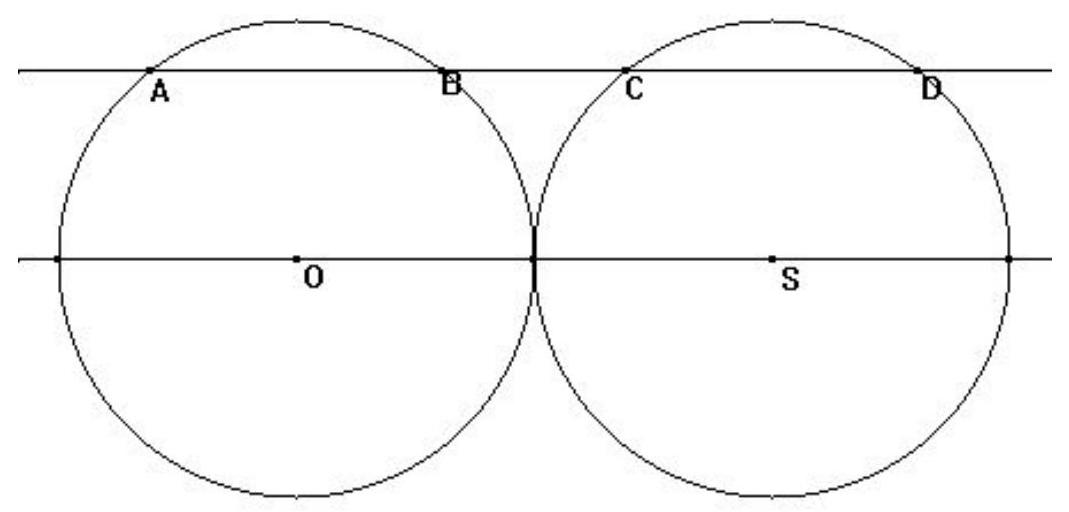
\includegraphics[max width=\textwidth, center]{2024_11_21_2558362c2bd32ec13884g-1(1)}

Zad. 3 Bartek ma pewną liczbę ołowianych żołnierzyków. Kiedy spróbował ustawić ich czwórkami, to zostało mu trzech. Gdy spróbował ustawić ich trójkami, to zostało mu dwóch. Ile żołnierzyków mu zostanie, jeśli swoje wojsko będzie ustawiał szóstkami?

Zad. 4 Dane są liczby \(a, b, c, x\). Wiedząc, że \(a+b+c=13\) oraz \(a x+b x+c x=169\), oblicz \(2005 \cdot x\).\\
Zad. 5 Prostokąt podzielono dwoma odcinkami na cztery mniejsze prostokąty. Pola trzech prostokątów są równe 6, 4, 2, jak na rysunku. Oblicz pole całego prostokąta.\\
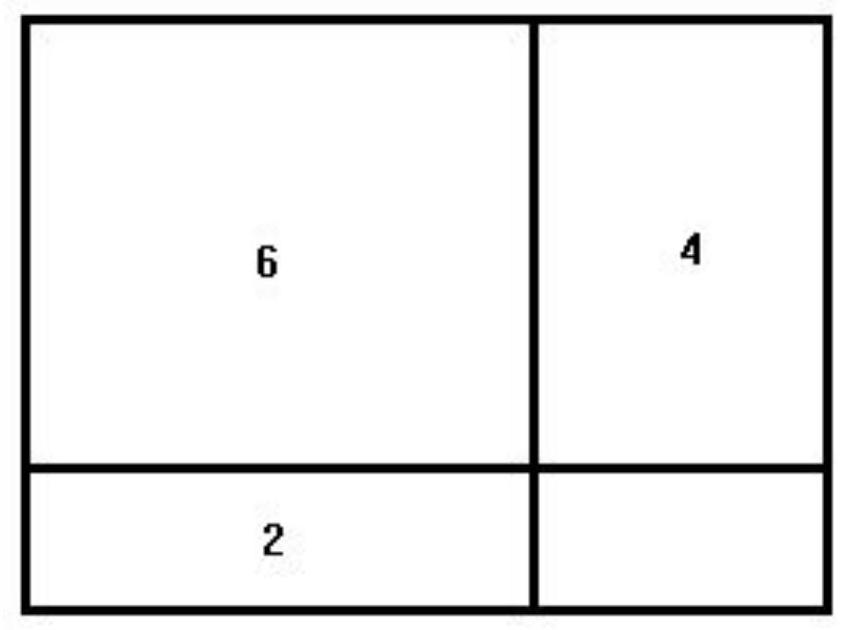
\includegraphics[max width=\textwidth, center]{2024_11_21_2558362c2bd32ec13884g-1}


\end{document}